% Chapter 1

\chapter{Introducción General} % Main chapter title

\label{Chapter1} % For referencing the chapter elsewhere, use \ref{Chapter1} 
\label{IntroGeneral}

%----------------------------------------------------------------------------------------

% Define some commands to keep the formatting separated from the content 
\newcommand{\keyword}[1]{\textbf{#1}}
\newcommand{\tabhead}[1]{\textbf{#1}}
\newcommand{\code}[1]{\texttt{#1}}
\newcommand{\file}[1]{\texttt{\bfseries#1}}
\newcommand{\option}[1]{\texttt{\itshape#1}}
\newcommand{\grados}{$^{\circ}$}

%----------------------------------------------------------------------------------------

%\section{Introducción}

En este capítulo se presenta una descripción del proceso que COPELECT realiza para obtener información sobre el consumo eléctrico de sus abonados, nociones sobre medidores inteligentes, una comparación de las soluciones comercialmente disponibles en esta temática, las razones que motivaron al desarrollo del trabajo junto con sus objetivos y alcances.

%----------------------------------------------------------------------------------------

\section{Medición del consumo eléctrico domiciliario}

En los hogares se dispone de diversos dispositivos eléctricos y electrónicos que son utilizados para entretenimiento, labores domésticas, trabajo, etc. La energía eléctrica consumida por estos dispositivos es medida en vatio-hora, simbolizado Wh \citep{WEBSITE:1}. El kWh, equivalente a 1000 vatios-hora, se utiliza para la facturación del consumo de energía eléctrica por parte de las compañías prestadoras del servicio \citep{WEBSITE:1}. Para este fin, las compañías instalan en los hogares de sus abonados dispositivos llamados medidores, que se encargan de contar la cantidad de kWh consumidos. También, los medidores proporcionan una interfaz para que los funcionarios de dichas compañías puedan registrar la información de consumo eléctrico.

Las mayor parte de compañías prestadoras del servicio eléctrico utilizan principalmente dos tipos de medidores para medir el consumo eléctrico domiciliario. Estos son:

\begin{enumerate}
	\item Medidores analógicos: contienen un disco giratorio metálico y un contador analógico que indica el total de kWh consumidos. Cuando la corriente fluye a través del medidor, se genera un campo eléctrico que impulsa el disco a girar. Entonces, la velocidad angular del disco está relacionada linealmente con el consumo eléctrico. Cada medidor analógico tiene un valor que indica el número de revoluciones que representan exactamente 1 kWh \citep{WEBSITE:2}.
	\item Medidores digitales: tienen una interfaz que consiste en una pequeña pantalla digital para mostrar la cantidad total de kWh consumidos y una salida de pulso óptico compuesta por un LED (\textit{Light-Emitting Diode}). Cada cierta cantidad de transiciones entre el estado apagado y encendido del LED representa exactamente 1 kWh consumido, esta cantidad es una constante indicada por el medidor como impulsos/kWh. Por lo tanto, monitorear el parpadeo del LED brinda la capacidad obtener el consumo eléctrico en el tiempo. El valor de los impulsos/kWh difiere según el fabricante del medidor y generalmente se encuentra debajo del LED \citep{WEBSITE:2}.
\end{enumerate}

En las figuras 1.1 y 1.2, se pueden observar un medidor de consumo eléctrico analógico y otro digital, respectivamente.

\begin{figure}[h]
	\centering
	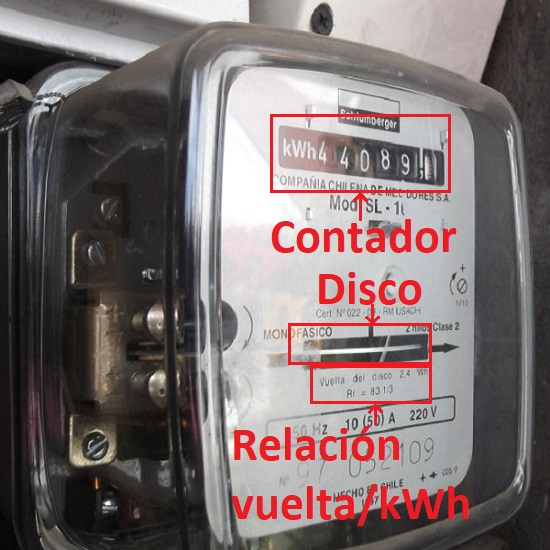
\includegraphics[scale=0.35]{./Figures/analog_meter.jpg}
	\caption{ Medidor de consumo eléctrico analógico.}
	\label{fig:cuadradoAzul}
\end{figure}

\begin{figure}[h]
	\centering
	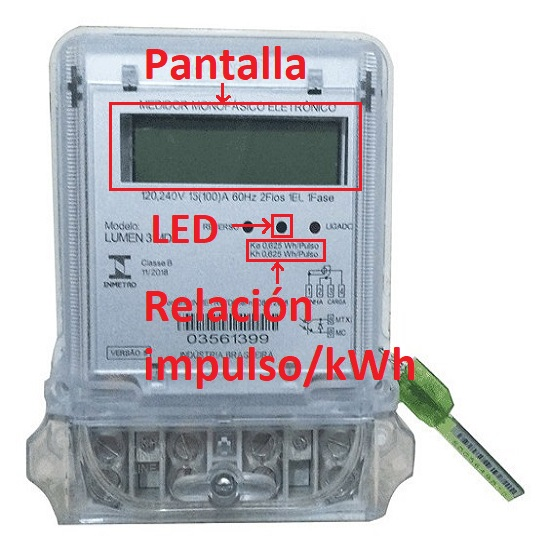
\includegraphics[scale=0.55]{./Figures/digital_meter.jpg}
	\caption{ Medidor de consumo eléctrico digital.}
	\label{fig:cuadradoAzul}
\end{figure}

Cuando la compañía prestadora del servicio eléctrico quiere obtener la información de consumo de sus medidores, lo hace registrando el valor que exhibe la interfaz del medidor, que posee un contador analógico en el caso de un medidor analógico o una pantalla digital en el caso de un medidor digital, ambas exhiben el total de kWh consumidos por el abonado.

La cooperativa de servicios eléctricos Tupiza Ltda., COPELECT, de la ciudad de Tupiza, Bolivia, tiene instalados alrededor de diez mil medidores de consumo eléctrico analógicos y digitales de uso domiciliario en los hogares de sus abonados, que son monitoreados para determinar el consumo eléctrico de cada uno de ellos. El monitoreo lo realizan funcionarios que se desplazan por toda la ciudad y registran el valor que exhibe la interfaz de los medidores junto con el nombre del abonado al que corresponde. Esta información es recopilada y utilizada para emitir la factura correspondiente de cada abonado. Finalmente, la factura emitida es impresa y llevada por los funcionarios a los hogares de los abonados para que tengan conocimiento del monto que deben pagar por su consumo eléctrico.

El proceso de monitoreo antes descrito es llevado a cabo una vez al mes por doce funcionarios, quienes tardan alrededor de ocho días en registrar toda la información de los medidores. Posteriormente, esa información es introducida a una base de datos que funciona en un servidor local ubicado en las oficinas centrales de COPELECT. La cantidad de kWh consumidos que deben ser facturados se determinan al restar el conteo de kWh del mes anterior con el actual. En casos particulares donde los funcionarios no pueden acceder al medidor para registrar el conteo de kWh consumidos, se emite la factura con los datos del mes anterior.

%----------------------------------------------------------------------------------------

\section{Medición inteligente}

La mayoría de los medidores de consumo eléctrico utilizados por parte de las compañías que prestan dicho servicio, sean estos analógicos o digitales, son dispositivos cuya única función es medir y exhibir mediante su interfaz la cantidad de kWh consumidos. Esta información únicamente es útil para la compañía y no brinda otros datos de relevancia. Existen también en el mercado otro tipo de medidores cuyas prestaciones son beneficiosas tanto para la compañía como para el abonado.

Los medidores inteligentes o \textit{smart meters}, son dispositivos que graban información como el consumo eléctrico, niveles de voltaje, corriente y factor de potencia. Esta información es comunicada a la compañía eléctrica para generar la facturación de sus servicios y a los abonados para que tengan mayor conocimiento sobre el comportamiento de su consumo eléctrico. Los smart meters típicamente graban la información eléctrica en tiempo real o en intervalos cortos a lo largo del día.

En la figura 1.3 se observa un smart meter.

\begin{figure}[h]
	\centering
	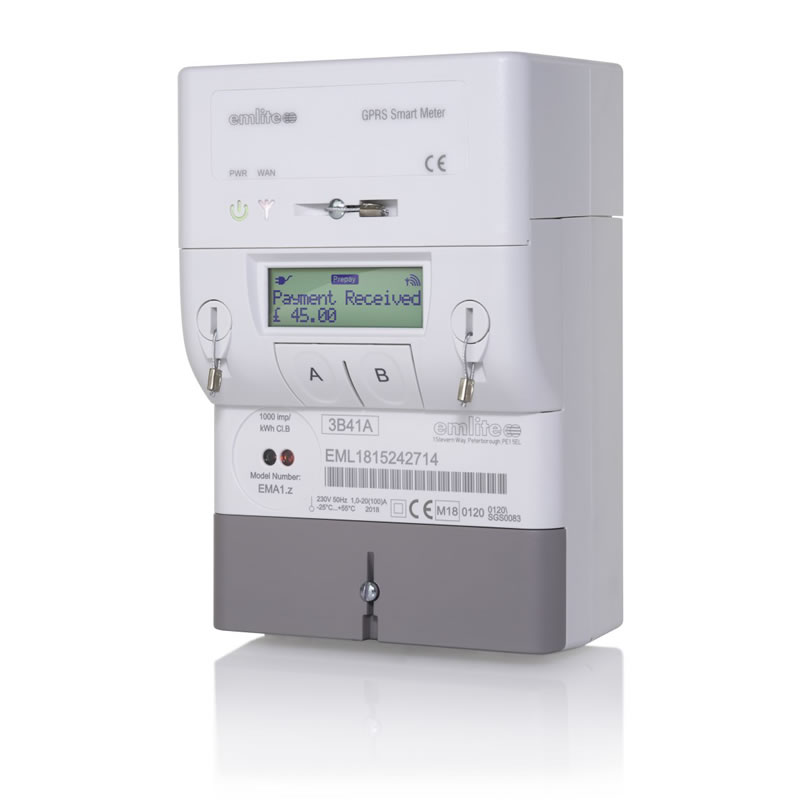
\includegraphics[scale=0.31]{./Figures/smart_meter.jpg}
	\caption{Smart meter de la firma emlite.}
	\label{fig:cuadradoAzul}
\end{figure}

Para mejorar el proceso de monitoreo y adquisición de información sobre consumo eléctrico, los smart meters representan una solución idónea, pero, el costo de su implementación los vuelve inviables para muchas compañías que ofrecen el servicio eléctrico. Entonces, debido a la problemática antes planteada, existe un mercado creciente para medidores no inteligentes, ampliados con un dispositivo que transfiere la información sobre el consumo eléctrico a la compañía y al abonado.

El dispositivo añadido a los medidores eléctricos de uso convencional puede utilizar distintos tipos de sensores para obtener la información de consumo eléctrico. Estos son:

\begin{itemize}
	\item Pinza de corriente: es una bobina sujeta alrededor de un conductor eléctrico. Cuando la corriente pasa a través del conductor, se genera un campo eléctrico. La bobina medirá este campo eléctrico y lo traducirá  a un flujo de corriente \citep{WEBSITE:3}.
	\item Cámara: podría ser situada en frente de del medidor y periódicamente tomar obtener fotografías del contador o pantalla. Las lecturas del consumo pueden ser extraídas de estas fotografías con técnicas de procesamiento de imágenes \citep{ARTICLE:1}.
	\item Foto-reflector: consiste en un LED y un fototransistor en una sola carcasa. Este sensor es posicionado en frente del disco que poseen los medidores analógicos, cuando el LED emite luz es reflejada por el disco y medida por el fototransistor \citep{WEBSITE:4}.
	\item Fototransistor: en conjunto con la salida de pulso óptico de los medidores digitales, se puede contar la cantidad de veces que el LED pasa de estado bajo a alto, para determinar el consumo eléctrico \citep{WEBSITE:5}.
\end{itemize}

%----------------------------------------------------------------------------------------

\section{Soluciones disponibles en el mercado}

Como se mencionó en la subsección anterior, dotar a los medidores convencionales de un dispositivo que amplíe sus funciones, es una manera de mejorar el proceso de monitoreo y adquisición de información de consumo eléctrico que realizan las compañías prestadoras de servicio.

Comercialmente existen dispositivos que cumplen esta función y utilizan alguno de los sensores adecuados para este fin. La fabricación de estos dispositivos se realiza sobre todo en Estados Unidos y algunos países europeos. A continuación se listan algunos dispositivos que utilizan la salida de pulso óptico de los medidores digitales para registrar el consumo de kWh:

\begin{itemize}
	\item PA-FL \citep{WEBSITE:6} es un contador de pulsos con comunicación inalámbrica de la firma SyxthSense. Es alimentado mediante baterías o una fuente de tensión de 24 V y trabaja como parte de un sistema propietario de SyxthSense. Puede ser instalado en medidores de electricidad, agua o gas y transmitir inalámbricamente los datos que registra utilizando una modulacion de tipo FSK (\textit{Frequency Shift Keying}) en la banda de 868.3 MHz. También, posee dos salidas de potencia de 1 A y y 60 V que pueden ser utilizadas para interactuar con otros dispositivos eléctrico o electrónicos. Dispone de una carcasa con certificación IP54. En la figura 1.4 se muestra una fotografía del dispositivo.
	
	\begin{figure}[h]
		\centering
		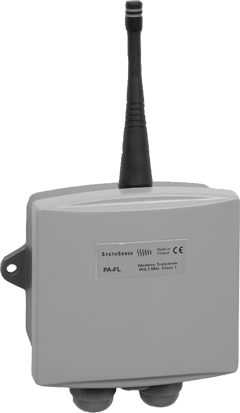
\includegraphics[scale=0.5]{./Figures/PA-FL.png}
		\caption{Registrador de pulsos PA-FL de la firma SyxthSense.}
		\label{fig:cuadradoAzul}
	\end{figure}

	\item AirTM-100S \citep{WEBSITE:7}: creado por la firma iNES, es un dispositivo diseñado para adquirir datos de medidores de energía eléctrica, agua y gas. Utiliza la salida de pulso óptico de medidores digitales para registrar el consumo del servicio. Es alimentado por una batería de 3.6 V que le brinda un tiempo de vida de aproximadamente cinco años, tiene carcasa con certificación IP65 y puede transmitir utilizando redes SIGFOX \footnote{SIGFOX. Es un operador de red global fundado en 2009, que implementa redes inalámbricas para conectar dispositivos de bajo consumo como pueden ser medidores eléctricos, centrales de alarmas o relojes inteligentes.}  a una frecuencia de 868 MHz. El dispositivo puede observarse en la figura 1.5.
	
	\begin{figure}[h]
		\centering
		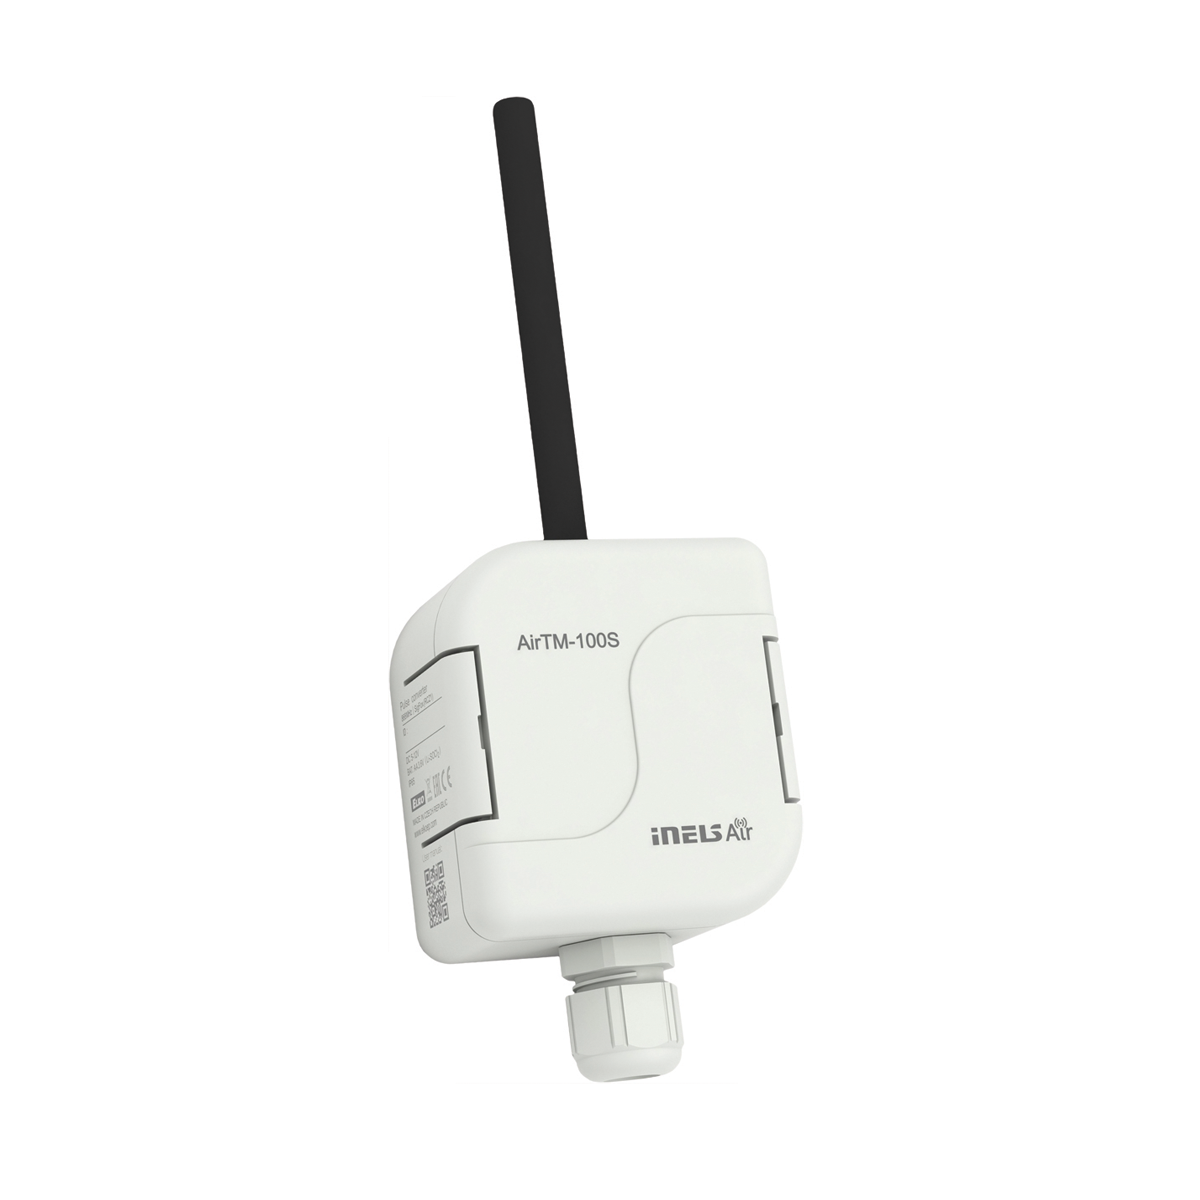
\includegraphics[scale=0.22]{./Figures/airtm-100s.png}
		\caption{Registrador de pulsos AirTM-100S de la firma iNES.}
		\label{fig:cuadradoAzul}
	\end{figure}	
\end{itemize}

%----------------------------------------------------------------------------------------

\section{Motivación}

Hoy en día, no solo las compañías de servicio eléctrico están interesadas en los números que proporcionan los medidores domiciliarios, sino también los propios abonados. Con la introducción del \textit{smart meter}, la cantidad de electricidad consumida se puede comunicar en tiempo real al abonado. Este consumo se presenta en un dispositivo, por ejemplo, un teléfono inteligente o una tableta, que brinda más información a los abonados y los motiva a reducir su consumo de energía hasta en un 9\% \citep{WEBSITE:8}.Entonces, el trabajo se originó como una propuesta de COPELECT, para contar con una alternativa tecnológica que optimice el proceso de monitoreo de los medidores que tiene instalados en la ciudad boliviana de Tupiza y proporcione a sus usuarios una manera de conocer su consumo eléctrico de manera oportuna.

Otra motivación importante para la realización de este trabajo fue la aplicación de los conocimientos adquiridos en la carrera de Especialización, para desarrollar e implementar un dispositivo basado en buenas prácticas de desarrollo de \textit{firmware} y \textit{hardware}, que sea lo suficientemente robusto y eficiente para que puedan reproducirlo por cientos o miles de unidades.

%----------------------------------------------------------------------------------------

\section{Objetivos y alcance}

El objetivo principal de este trabajo fue desarrollar e implementar un dispositivo electrónico, capaz de monitorear un medidor de consumo eléctrico de uso domiciliario mediante la salida de pulso óptico incorporada, para proporcionar la información obtenida a la compañía prestadora del servicio de manera remota y permitir al abonado conocer su consumo eléctrico en el momento que realiza la consulta a través de una interfaz gráfica web.

El alcance de este proyecto incluye:

\begin{itemize}
	\item Un prototipo comercial que pueda ser instalado en los medidores de consumo eléctrico de COPELECT.
	\item Manual de uso e instalación.
\end{itemize}